\documentclass[10pt,a4paper]{article}
\usepackage[margin=0.5cm]{geometry}
\usepackage[utf8]{inputenc}
\usepackage[english]{babel}
\usepackage{amsmath}
\usepackage{amsfonts}
\usepackage{amssymb}
\usepackage{graphicx}
\usepackage{epstopdf}
\usepackage{epsfig}
\usepackage[font=footnotesize]{subfig}
\usepackage{hyperref}
\usepackage{eufrak}
\usepackage{xcolor}
\graphicspath{ {./img/} }

%\documentclass[a4paper]{article}
%\usepackage[english]{babel}
%
%\usepackage{graphicx}
%
%\let\ifpdf\relax
%\usepackage[font=footnotesize]{subfig}
%\usepackage{hyperref}
%\usepackage{graphicx}
%\usepackage{epsfig}
%\usepackage{epstopdf}
%\usepackage{amsmath}
%\usepackage{eufrak}
%\usepackage{xcolor}


\author{autogenerated by MDSip-test tools}
\title{MDSip throughput tests report}




\begin{document}

\maketitle

\section{ Optimal segment size vs protocol }

Tests has been performed using different algorithms TCP and UDT. The testing software talks to a 10Gbps connected machine located at nifs (\emph{test10g.nifs.ac.jp}). This target endpoint and has been opened for connections coming from \emph{ra22.igi.cnr.it} (Red Hat Enterprise Linux Server release 5.1) server at RFX.

\begin{figure}[htbp!]
\centerline{
\subfloat[]{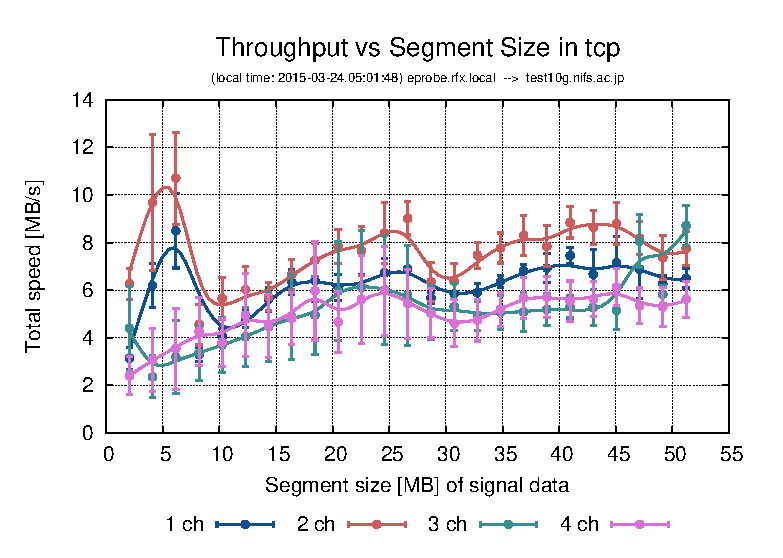
\includegraphics[width=0.5\textwidth]{img/size-tcp.eps} \label{fig:fig1} }
\subfloat[]{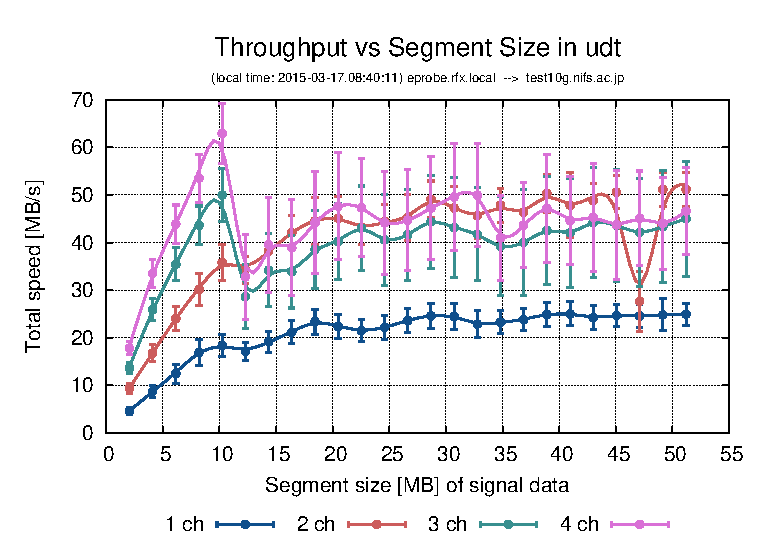
\includegraphics[width=0.5\textwidth]{img/size-udt.eps} \label{fig:fig1} }
}
\caption[]
{ TCP vs UDT connection throughput }
\label{fig:size}
\end{figure}

\begin{figure}[htbp!]
\centerline{
\subfloat[]{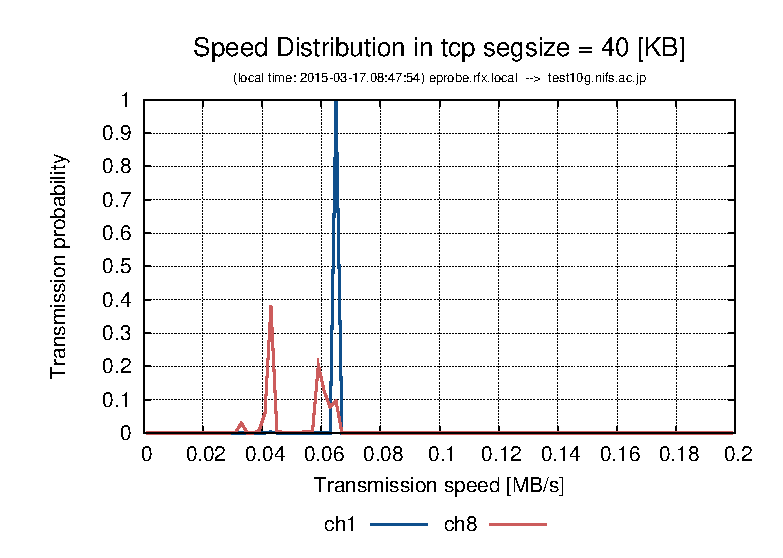
\includegraphics[width=0.5\textwidth]{img/distr-tcp-speed.eps} \label{fig:fig1} }
\subfloat[]{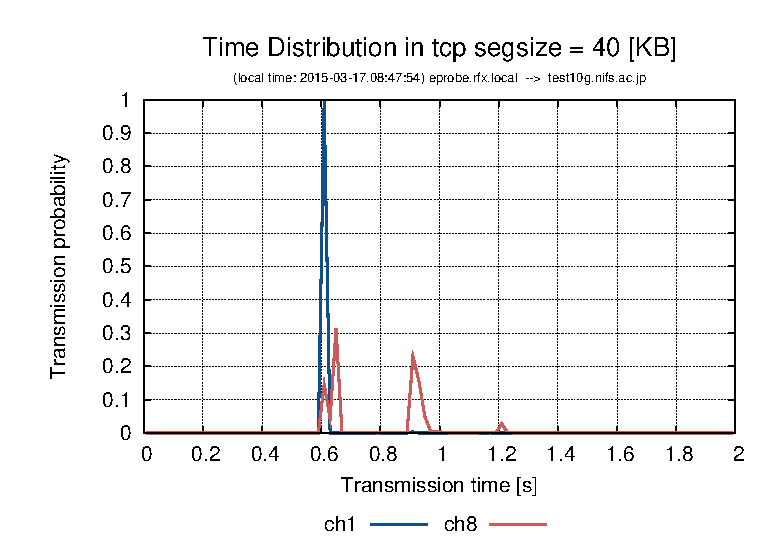
\includegraphics[width=0.5\textwidth]{img/distr-tcp-time.eps} \label{fig:fig1} }
}
\caption[]
{ Timing distributions for TCP connection }
\label{fig:distr-tcp}
\end{figure}


\begin{figure}[htbp!]
\centerline{
\subfloat[]{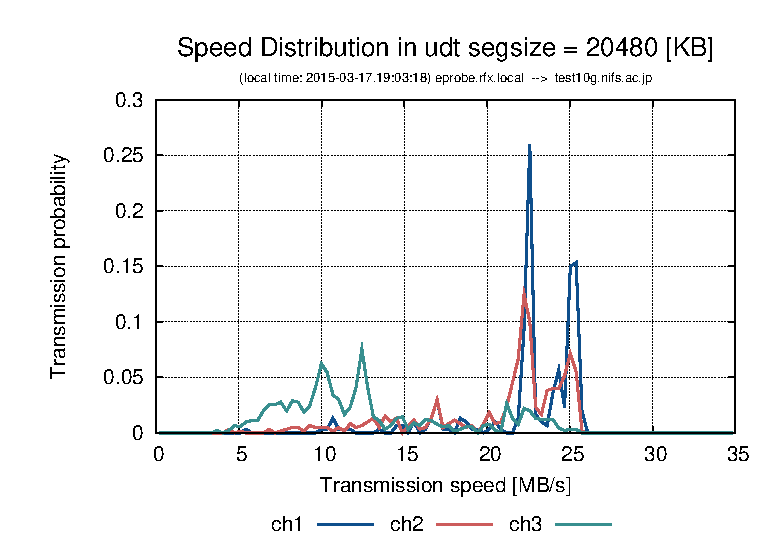
\includegraphics[width=0.5\textwidth]{img/distr-udt-speed.eps} \label{fig:fig1} }
\subfloat[]{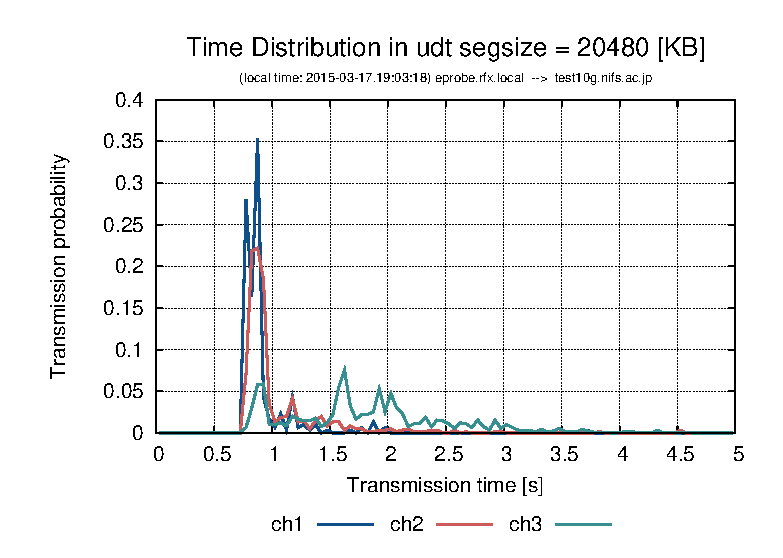
\includegraphics[width=0.5\textwidth]{img/distr-udt-time.eps} \label{fig:fig1} }
}
\caption[]
{ Timing distributions for UDT connection }
\label{fig:distr-udt}
\end{figure}







\end{document}